\documentclass[hyperref]{beamer}
\usepackage{beamerthemesplit}
\usepackage{graphicx}
\usepackage{mathptmx}           % replacement for obsolete \usepackage{times}
\usepackage[scaled=.90]{helvet} % replacement for obsolete \usepackage{times}
\usepackage{courier}            % replacement for obsolete \usepackage{times}

\usepackage{tikz}
\usetikzlibrary{shapes.arrows,chains,positioning,automata,trees,calc}
\usetikzlibrary{patterns}
\usetikzlibrary{decorations.pathmorphing,decorations.markings}
\usepackage{times,latexsym,amsfonts,amssymb,amsmath,graphicx,url,bbm,rotating,siunitx}
\usepackage{multirow,hhline,arydshln,array,color,stmaryrd}
\definecolor{darkred}{rgb}{0.5, 0.0, 0.0}
\definecolor{darkgreen}{rgb}{0.0, 0.4, 0.0}
\definecolor{darkblue}{rgb}{0.0, 0.0, 0.5}

% set up Beamer style with Stanford colors and logo
% logo is available at http://nlp.stanford.edu/local/nlp-logos/nlp-logo.pdf
\useinnertheme{rounded}
\useoutertheme{infolines}
\usecolortheme{beaver}
\setbeamercolor{block title}{fg=white,bg=darkred!75!black}
\setbeamercolor{block body}{parent=normal text,bg=black!5!bg}
\setbeamercolor{item projected}{bg=darkred}
\logo{
\includegraphics[height=1cm]{../img/nlp-logo.pdf}}

% title page information
\title{Relation Extraction As Inference}
\subtitle{}
\author{Gabor Angeli, Chris Manning}
\date{January 5, 2015}
\institute[Stanford]{Stanford University}

\input ../macros.tex
\input ../figures.tex

\begin{document}
\begin{frame}
  \titlepage
\end{frame}

%%%%%%%%%%%%%%%%%%% 
% RELATION EXTRACTION
%%%%%%%%%%%%%%%%%%%
\begin{frame}{Relation Extraction}
\begin{tabular}{rl}
  \textbf{Input:} & \w{Chris, a tenured professor at Stanford, is friends with Fei-Fei.} \\
                  & (4 million other sentences) \\
                    \pause
                    \hspace{1em}
  \textbf{Output:} & ( Chris, per:employee\_of, Stanford )
\end{tabular}
\pause

\vspace{1cm}
\begin{center}
  
\includegraphics[scale=0.25]{../img/google-now-voice.png} \\
  OK Google, where does Chris work?
\end{center}
\end{frame}

%%%%%%%%%%%%%%%%%%% 
% CLASSIFICATION
%%%%%%%%%%%%%%%%%%%
\begin{frame}{Standard Approach: Classification}
\hh{Dataset:}
\begin{itemize}
  \item (\w{Chris, a professor at Stanford, is friends with Fei-Fei}, \textbf{employee\_of})
  \item (\w{Chris is not a professor at Berkeley}, \textbf{none})
  \item $\dots$
\end{itemize}
\vspace{0.5cm}

\hh{$k$-way Classification Task}
%\begin{itemize}
%  \item Dependency features, surface features, distributional features, etc. 
%  \item Noisy data, but works well anyways.
%\end{itemize}
\pause
\vspace{0.5cm}

\hh{Great! Why do anything else?}
\begin{itemize}
  \item only works on $k$ classes.
        What about ``can\_be\_picked\_up\_by?''
  \item ``High'' recall (0.29), but low precision (0.36).
  \item Easily thrown off by subtleties (e.g., \w{not}).
\end{itemize}
\end{frame}

%%%%%%%%%%%%%%%%%%% 
% ENTAILMENT
%%%%%%%%%%%%%%%%%%%
\begin{frame}{Treat As Entailment}
\begin{center}
  \w{Chris, a tenured professor at Stanford, is friends with Fei-Fei} \\ $\Rightarrow$ \w{Chris is employee of Stanford}
\end{center}

\hh{Step 1:} Split sentence into clauses
\begin{itemize}
  \item[] \w{Chris is a tenured professor at Stanford}
  \item[] \w{Chris, a tenured professor at Stanford, is friends with Fei-Fei}
\end{itemize}
\pause

\hh{Sometimes challenging:}
\begin{center}
  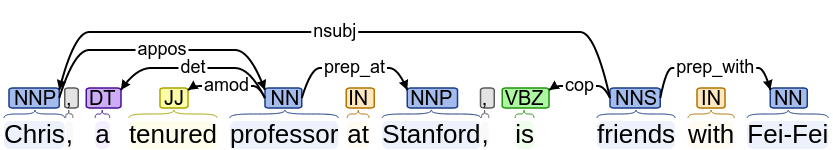
\includegraphics[scale=0.33]{../img/tree-chris-feifei.png}
\end{center}

\hh{Approach:} Train classifier for whether a dependency arc is a clause.

\end{frame}

\begin{frame}{Treat As Entailment}
\begin{center}
  \w{Chris, a tenured professor at Stanford, is friends with Fei-Fei} \\ $\Rightarrow$ \w{Chris is employee of Stanford}
\end{center}

\hh{Step 1:} Split sentence into clauses \\
\hh{Step 2.1:} Entailment (forward) -- Natural Logic
\begin{itemize}
  \item[] \w{Chris is a tenured professor at Stanford}
    \begin{itemize}
      \item[$\Rightarrow$] Chris is a tenured professor
      \item[$\Rightarrow$] Chris is a professor at Stanford
      \item[$\Rightarrow$] Chris is at Stanford
    \end{itemize}
  \item[] \w{Chris, a professor at Stanford, is friends with Fei-Fei}
    \begin{itemize}
      \item[$\Rightarrow$] Chris is friends with Fei-Fei
      \pause
      \item[$\Rightarrow$] \darkred{* \textit{Chris is friends}}
    \end{itemize}
\end{itemize}

%\pause
%\hh{Natural Logic!}
%\begin{itemize}
%  \item But, with a bit of care for prepositional clauses. \\
%\end{itemize}
\end{frame}

\begin{frame}{Treat As Entailment}
\begin{center}
  \w{Chris, a tenured professor at Stanford, is friends with Fei-Fei} \\ $\Rightarrow$ \w{Chris is employee of Stanford}
\end{center}

\hh{Step 1:} Split sentence into clauses \\
\hh{Step 2.1:} Entailment (forward) \\
\hh{Step 2.2:} Entailment (reverse)
\begin{itemize}
  \item NaturalLI (Natural Logic for Common Sense Reasoning)
  \pause
  \item[] $+$ relational entailment: \w{is at} $\Rightarrow$ \w{is employee of}
  \pause
  \item[] $+$ meronymy \w{born in Hawaii} $\Rightarrow$ \w{born in USA}
  \pause
  \item Open-domain: still works for common-sense facts.
\end{itemize}
\pause

\vspace{0.5cm}
\begin{center}
  \large{Thanks!}
\end{center}
\end{frame}

\end{document}



